\subsubsection{Part 2:}

This section introduces larger numbers of users, testing with 1, 5, 10, 20, and
50 users. This testing was implemented, as with every section, using a bash
script, which can be found in the Appendices. As the loop implemented in the
previous section allows for any amount of users to be input, the bash script
simply needs to execute the simulation for each of the desired number of users.

\begin{lstlisting}[language=Bash, caption=wifi-p1qcp2.sh File Snippet]

USERS="1 5 10 20 50"

#Code Removed for purposes of snippet

  for user in $USERS
   do
    echo Trial $trial, Users $user
     ../../waf --run "WiFi --users=$user --dbPrefix=$DBPREFIX --txInterval=$TXINTERVAL --run=run-$trial-$DBPREFIX-$user"
   done
\end{lstlisting}

The throughput can be seen to be relatively robust for each number of users,
with each case having approximately 1Mbps throughput. The 20 and 50 user systems
have slightly less than 1Mbps, however, as the difference is minor, it is not
easily visible in the plot.

\begin{gather*}
	Throughput=\frac{rxPackets*1000*8}{txTime} \\
	TP_{1-10 Users}= 1000Kbps\\
	TP_{20 Users}= \frac{1686.45*1000*8}{20}\\
	= 647.58Kbps (\text{using average number of rxPackets}) \\
	TP_{20 Users} = 989.92Kbps (\text{using Bash Script}) \\
	TP_{50 User}= 989.92Kbps (\text{using Bash Script}) \\
\end{gather*}

\begin{figure}[H]
	\centering
	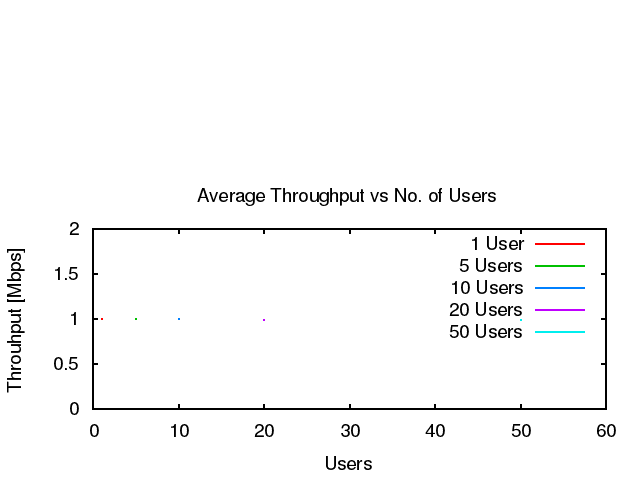
\includegraphics[width=0.8\textwidth]{images/EE500/QC/P2/Images/wifi-throughput}
	\caption{Throughput for systems with 0 to 50 users}
	\label{fig:QCP2throughput}
\end{figure}

The delay increases from a value of 0.44ms in a single user system to
approximately 1530ms for a 50 user system. This can be seen in Figure
\ref{fig:QCP2delay}. The equations below show the values as extracted from the
.db file using the bash script.

\begin{gather*}
	\overline{delay}=\frac{delaySum}{rxPackets} \\
	\overline{delay}_{1 User}=441013ns \\
	\overline{delay}_{5 User}=2807059ns \\
	\overline{delay}_{10 User}=8420910ns \\
	\overline{delay}_{20 User}=277970000ns \\
	\overline{delay}_{50 User}=1530570000ns \\
\end{gather*}

\begin{figure}[H]
	\centering
	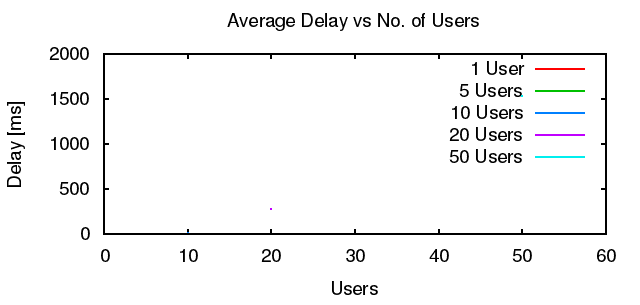
\includegraphics[width=0.8\textwidth]{images/EE500/QC/P2/Images/wifi-delay}
	\caption{Delay for systems with 0 to 50 users}
	\label{fig:QCP2delay}
\end{figure}

The systems relative robustness can also be shown through its packet loss ratio
values for all numbers of users. For 1 to 10 users, there are no lost packets.
For the 20 and 50 user systems, there is a PLR of only 1.08\%, as extracted from
the .db file.

\begin{gather*}
	PLR=\frac{lostPackets}{rxPackets+lostPackets} \\
	PLR_{1 User}=0 \\
	PLR_{5 User}=0 \\
	PLR_{10 User}=0 \\
	PLR_{20 User}=1.08\% \\
	PLR_{50 User}=1.08\% \\
\end{gather*}

\begin{figure}[H]
	\centering
	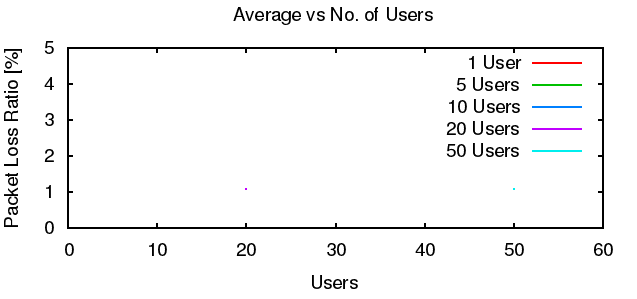
\includegraphics[width=0.8\textwidth]{images/EE500/QC/P2/Images/wifi-loss}
	\caption{Loss for systems with 0 to 50 users}
	\label{fig:QCP2loss}
\end{figure}
